\documentclass[11pt]{beamer}
\usetheme{Szeged}
\usecolortheme{dolphin}
\usefonttheme[onlymath]{serif}

\usepackage{graphicx} \usepackage{url} \usepackage{hyperref} \usepackage{caption} \usepackage{amsmath}
\usepackage{amssymb} \usepackage{array} \usepackage{listings} \usepackage{color} \usepackage{textcomp}
\usepackage[utf8]{inputenc} \usepackage{natbib} \usepackage{algorithm} \usepackage{tikz}
\usepackage[noend]{algpseudocode} \usepackage{csquotes}

\usetikzlibrary{shapes.geometric, arrows}

\setbeamercovered{transparent}
\setbeamertemplate{navigation symbols}{}
\setbeamerfont{page number in head/foot}{size=\fontsize{9}{11}}
\setbeamertemplate{footline}[frame number]
\setbeamertemplate{section in toc}{\inserttocsectionnumber.~\inserttocsection}

\author{Glenn Galvizo}
\title{Experiment Overview: Benchmarking Neo4J and Apache Cassandra for Common Stellar Queries}
\institute{University of Hawaii at Manoa \\ ICS 421}

\begin{document}
    \begin{frame}
        \titlepage
    \end{frame}

    \begin{frame}
        \frametitle{Overview}
        \tableofcontents
    \end{frame}

    \section{Background}\label{sec:background}
    \subsection{Introduction}\label{subsec:introduction}
    \begin{frame}
        \frametitle{Roots: Ancient Navigation}
        \centerline{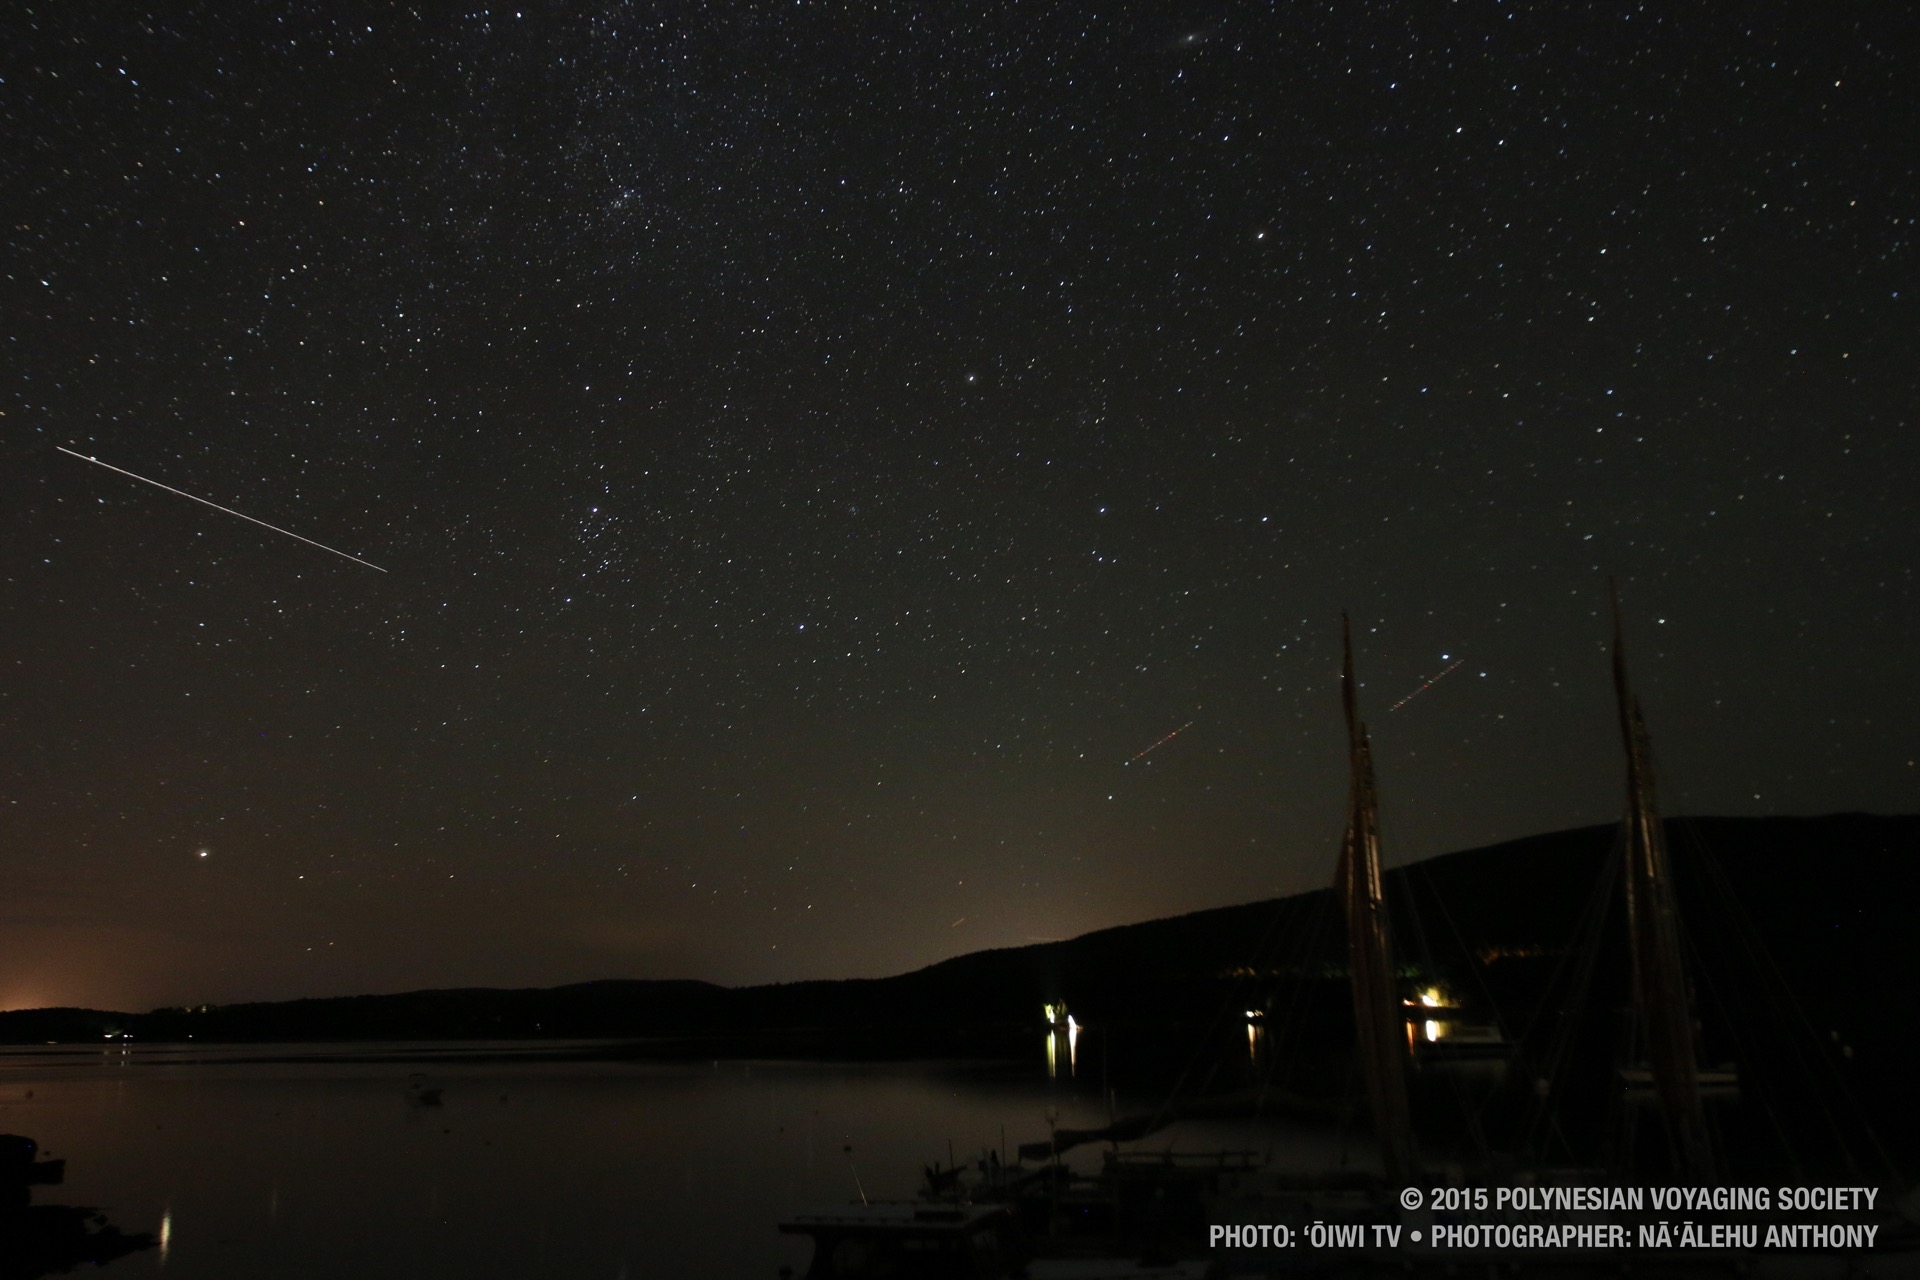
\includegraphics[scale=0.18]{images/hokulea.jpg}}
    \end{frame}

    \subsection{Problem Statement}\label{subsec:problemStatement}
    \begin{frame}
        \frametitle{Problem Statement}
        \begin{block}{Questions of Interest (Queries)}
            \begin{enumerate}
                \item What are the characteristics of some star $s$? \medskip
                \item What stars are near some star $s$? \medskip
                \item What stars are near some position $(\alpha, \delta)$? \medskip
                \item What stars are near some position $(\alpha, \delta)$ AND \\ below some magnitude (brightness)
                $m$? \medskip
                \item What stars are near some star $s$ AND \\ below some magnitude (brightness) $m$?
            \end{enumerate}
        \end{block} \medskip
        \begin{block}{Problem}
            \centerline{\textbf{How do we organize our catalog of stars for efficient access?}}
        \end{block}
    \end{frame}

    % https://vignette.wikia.nocookie.net/mrcameronsy11cosmologyclass/images/7/73/Map.gif/revision/latest?cb=20120926202437
    \subsection{Dataset}\label{subsec:dataset}
    \begin{frame}
        \frametitle{Tycho-2 Dataset}
        \begin{columns}
            \begin{column}{0.5\textwidth}
                \begin{enumerate}
                    \item 2.5 million stars \& attributes \medskip
                    \item Stars identified by \texttt{TYC1, TYC2, TYC3} \medskip
                    \item \texttt{TYC1} = Guide Star Region (GSC Number) \medskip
                    \item Sky divided into regions $3.75^\circ \times 3.75^\circ$ (\texttt{TYC1}) \medskip
                    \item \textit{Near star if in same region}
                \end{enumerate}
            \end{column}
            \begin{column}{0.5\textwidth}
                \centering{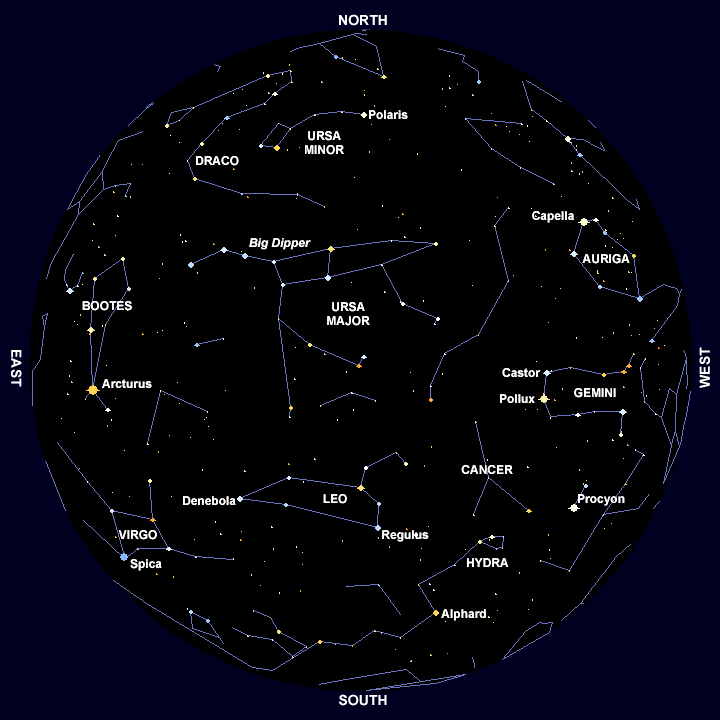
\includegraphics[scale=0.3]{images/skymap.png}}
            \end{column}
        \end{columns}
    \end{frame}

    \section{NoSQL Systems}\label{sec:noSQLDataModels}
    \subsection{Graph Data Systems}\label{subsec:graphDataModel}
    \begin{frame}
        \frametitle{Graph Data Model}
        \begin{columns}
            \begin{column}{0.5\textwidth}
                \begin{enumerate}
                    \item Nodes hold properties \bigskip
                    \item Edges define relationships between nodes \bigskip
                    \item Nodes + edges = graph \bigskip
                    \item Efficient queries traverse the graph(s)
                \end{enumerate}
            \end{column}
            \begin{column}{0.5\textwidth}
                \centering{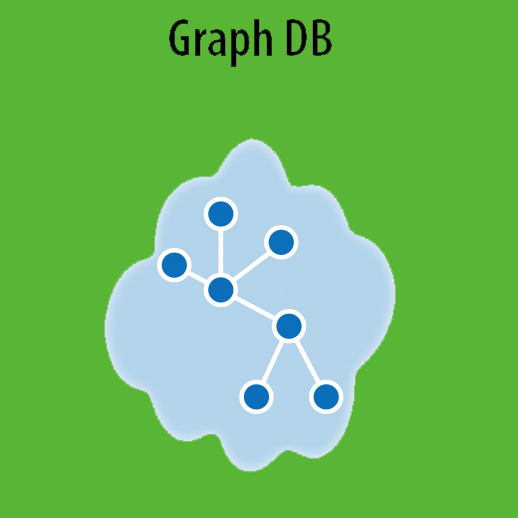
\includegraphics[scale=0.4]{images/graph-model.png}}
            \end{column}
        \end{columns}
    \end{frame}

    \begin{frame}
        \frametitle{Neo4J}
        \begin{columns}
            \begin{column}{0.5\textwidth}
                \begin{itemize}
                    \item = Distributed graph store \bigskip
                    \item Consistent, available, not partition-tolerant \bigskip
                    \item \textit{Data sharding not available} \bigskip
                    \item Project Data Model:
                    \begin{enumerate}
                        \item Nodes: Stars, Regions
                        \item Regions CONTAIN stars
                    \end{enumerate}
                \end{itemize}
            \end{column}
            \begin{column}{0.5\textwidth}
                \centerline{Cypher Nearby Query:}
                \begin{flalign*}
                    &\texttt{\footnotesize MATCH (s:Star)-[:CONTAINS]-(a:Region)} \\
                    &\texttt{\footnotesize WHERE 101.287 > a.RAmin } \\
                    &\texttt{\footnotesize \hspace*{1cm}AND 101.287 < a.RAmax} \\
                    &\texttt{\footnotesize \hspace*{1cm}AND -16.716 > a.DEmin} \\
                    &\texttt{\footnotesize \hspace*{1cm}AND -16.716 < a.DEmax} \\
                    &\texttt{\footnotesize RETURN s}
                \end{flalign*}
            \end{column}
        \end{columns}
    \end{frame}

    \subsection{Column Family Systems}\label{subsec:columnFamilyModel}
    \begin{frame}
        \frametitle{Column Family Model}
        \begin{columns}
            \begin{column}{0.5\textwidth}
                \begin{enumerate}
                    \item One property = one column \bigskip
                    \item Column indexed by \textit{primary} key \bigskip
                    \item Columns indexed by same key = column family \bigskip
                    \item Efficient queries use primary key
                \end{enumerate}
            \end{column}
            \begin{column}{0.5\textwidth}
                \centering{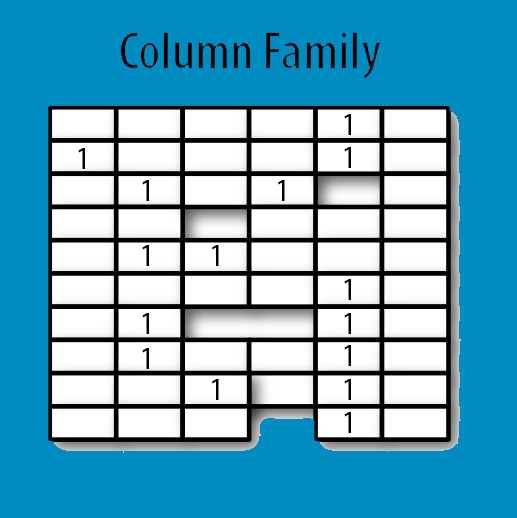
\includegraphics[scale=0.4]{images/column-model.png}}
            \end{column}
        \end{columns}
    \end{frame}

    \begin{frame}
        \frametitle{Apache Cassandra}
        \begin{columns}
            \begin{column}{0.5\textwidth}
                \begin{itemize}
                    \item = Distributed column store \bigskip
                    \item Available, partition-tolerant, not consistent \bigskip
                    \item Hash partitions data by primary key \bigskip
                    \item Project Data Model:
                    \begin{enumerate}
                        \item Column Families: Stars, Regions
                        \item Stars indexed by ID
                        \item Regions indexed by ID
                    \end{enumerate}
                \end{itemize}
            \end{column}
            \begin{column}{0.5\textwidth}
                \centerline{CQL Queries (Nearby, Naive):}
                \begin{align*}
                    t_i = \ &\texttt{\footnotesize SELECT TYC1} \\
                    &\texttt{\footnotesize FROM tycho.region} \\
                    &\texttt{\footnotesize WHERE RAmin < 101.287 } \\
                    &\texttt{\footnotesize \hspace*{1cm}AND RAmax > 101.287} \\
                    &\texttt{\footnotesize \hspace*{1cm}AND DEmin < -16.716} \\
                    &\texttt{\footnotesize \hspace*{1cm}AND DEmax > -16.716} \\
                    s = \ &\texttt{\footnotesize SELECT *} \\
                    &\texttt{\footnotesize FROM tycho.stars} \\
                    &\texttt{\footnotesize WHERE TYC1 = } t_i [0]
                \end{align*}
            \end{column}
        \end{columns}
    \end{frame}
    
    \section{Methodology}\label{sec:methodology}
    \begin{frame}
        \frametitle{Methodology}
        \begin{block}{Hardware}
            \begin{itemize}
                \item 1--3 Google Cloud nodes
                \item Node: 2vCPUs, 7.5GB memory
            \end{itemize}
        \end{block}
        \begin{block}{Testing Parameters}
            \begin{itemize}
                \item With/without index on filtered column
                \item Number of nodes in cluster used (1--3)
                \item Searching file for region ID
            \end{itemize}
        \end{block}
        \begin{block}{Measured}
            Time to execute queries, or query lists
        \end{block}
    \end{frame}

    \section{Conclusion}\label{sec:conclusion}
    \begin{frame}
        \frametitle{Conclusion}
        \begin{itemize}
            \item Finding nearby stars: $O(n)$ at worst \bigskip
            \item Graph databases use nodes and edges \bigskip
            \item Column store databases use columns \bigskip
            \item Goal: Measure the running time
        \end{itemize}
    \end{frame}

    \begin{frame}
        \centering{\huge{Questions?}}
    \end{frame}
\end{document}
